
% !TEX encoding = UTF-8 Unicode 
% !TEX root = FieldGuide.tex

\Sec{Beta Distribution}
\label{sec:Beta}




\dist{Beta} ($\beta$, Beta type I, Pearson type I) distribution~\cite{Pearson1895}:
\begin{align}
\label{Beta}
\opr{Beta}(x\given &a,s,\alpha, \gamma) \\
& = 
 \frac{1}{B(\alpha, \gamma)}\frac{1}{ \Left|s\Right|}
\Left(\frac{x-a}{s} \Right)^{\alpha -1} \Left (1-\Left(\frac{x-a}{s}\Right)\Right)^{\gamma -1}	\checked
\notag
\\ & = \opr{GenBeta}(x\given a,s,\alpha, \gamma,1) \notag						\checked
\end{align}
The beta distribution is one member of Person's distribution family, notable for having two roots located at the minimum and maximum of the distribution. The name arises from the beta function in the normalization constant.




% ====================================================================

\SSec{Special cases}
\phantomsection\addcontentsline{toc}{subsection}{~~~~~~~~~~~~U-shaped beta}
\phantomsection\addcontentsline{toc}{subsection}{~~~~~~~~~~~~J-shaped beta}
Special cases of the beta  distribution are listed in table~\ref{GenBetaTable}, under $\beta=1$.
With $\alpha<1$ and $\gamma<1$ the distribution is U-shaped with a single anti-mode ({\bf U-shaped beta} distribution). If $(\alpha-1)(\gamma-1)\leq 0$ then the distribution is a  monotonic {\bf J-shaped beta} distribution. 


\dist{Standard beta} (Beta) distribution: 
\begin{align}
\label{StdBeta}
\opr{StdBeta}(x\given \alpha, \gamma) &= 
 \frac{1}{B(\alpha, \gamma)} 
x^{\alpha-1} \Left (1- x\Right)^{\gamma -1}								\checked
\\ & = \opr{Beta}(x\given  0,1,\alpha,\gamma) \notag						\checked
\\ & = \opr{GenBeta}(x\given  0,1,\alpha,\gamma, 1) \notag				\checked
\end{align}
The standard beta distribution has two shape parameters, $\alpha>0$ and $\gamma>0$, and support $x\in[0,1]$. 

\begin{figure}[tp!]
\begin{center}
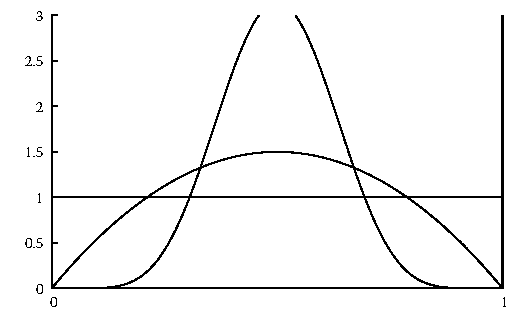
\includegraphics[width=\textwidth]{pdfBeta}
\end{center}
\caption[Beta distribution]{A beta distribution, $\opr{Beta}(0, 1, 2, 4)$}
\end{figure}

\dist{Pert} (beta-pert) distribution~\cite{Clark1962, Vose2000} is a subset of the beta distribution, parameterized by minimum ($a$), maximum ($b$) and mode ($x_\text{mode}$).  
\begin{align}
\label{Pert}
\opr{Pert}&(x\given a,b,x_\text{mode}) \checked
\\ \notag
&=  
 \frac{1}{B(\alpha, \gamma) (b-a)}
\Left(\frac{x-a}{b-a}\Right)^{\alpha-1} \Left(\frac{b-x}{b-a}\Right)^{\gamma-1} \checked
\\ \notag & \qquad x_\text{mean} = \frac{a+4x_\text{mode}+b}{6} \checked
%\\ & \qquad \alpha = 1 + 4 \frac{m-a}{b-a}, \quad \gamma = 1 + 4 \frac{b-m}{b-a}
\\ & \qquad \alpha = \frac{(x_\text{mean}-a)(2 x_\text{mode} - a - b)}{(x_\text{mode}-x_\text{mean})(b-a)} \checked
\notag 
\\\notag  & \qquad \gamma = \alpha\frac{(b-x_\text{mean})}{x_\text{mean}-a} \checked
\\ & = \opr{Beta}(x\given a,b-a,\alpha,\gamma) \checked \notag
\\ & = \opr{GenBeta}(x\given  a,b-a,\alpha,\gamma, 1)  \checked \notag
\end{align}
The PERT (Program Evaluation and Review Technique) distribution is used in project management to estimate task completion times. The {\bf modified pert} distribution replaces the estimate of the mean with $x_\text{mean}\! = \frac{a+\lambda x_\text{mode}+b}{2+\lambda}\checked$, where~$\lambda$ is an additional parameter that controls the spread of the distribution~\cite{Vose2000}.




% !TEX encoding = UTF-8 Unicode 
% !TEX root = FieldGuide.tex

\begin{table*}[tp]
\caption[Beta distribution -- Properties]{Properties of the beta distribution}
 \begin{align*}
 \text{\hyperref[PropertiesSec]{Properties}}  \quad& \\
\text{name} \quad & \op{Beta}(x\given a,s,\alpha, \gamma) 	\checked
\\
\text{PDF}\quad &    \frac{1}{B(\alpha, \gamma)}\frac{1}{ \Left|s\Right|}
\Left(\frac{x-a}{s} \Right)^{\alpha -1} \Left (1-\Left(\frac{x-a}{s}\Right)\Right)^{\gamma -1}	\checked
\hspace{-8em}
\\
\text{CDF / CCDF} \quad  & 
 \frac{B\Left( \alpha,\gamma; \sfrac{x-a}{s} \Right)}{B(\alpha,\gamma)} = I( \alpha,\gamma; \sfrac{x-a}{s})
 \checked
& {s} >0 \,\big/ \, {s} <0
\\ 
\text{parameters}\quad &   a,\ s,\ \alpha,\ \gamma, \text{ in } \Real, \\ &  \alpha,\gamma\geq0	\checked
\\
\text{support} \quad &  a \geq x \geq a+s , s>0 \quad a+s \geq x \geq a , s<0 
%\\
%\text{median} \quad   &  \cdots
\\
\text{mode} \quad  &a + s \frac{\alpha-1}{\alpha+\gamma-2}\checked  & \alpha,\gamma > 1
\\
\text{mean} \quad  &   a + s \frac{\alpha}{\alpha+\gamma}	\checked
\\
\text{variance} \quad   & s^2 \frac{\alpha\gamma}{(\alpha+\gamma)^2(\alpha+\gamma+1)} \checked
\\
\text{skew} \quad  &   \op{sgn}(s)\ \frac{2(\gamma-\alpha) \sqrt{\alpha+\gamma+1} }{(\alpha+\gamma+2)\sqrt{\alpha\gamma} } \checked
\\
\text{ex. kurtosis} \quad  &  6\frac{(\alpha-\gamma)^2(\alpha+\gamma+1) - \alpha\gamma(\alpha+\gamma+2) }{\alpha\gamma(\alpha+\gamma+2)(\alpha+\gamma+3)} \checked
\\
\text{entropy} \quad  &  \ln(|s|) + \ln\bigl(B(\alpha,\gamma)\bigr)-(\alpha-1)\psi(\alpha)
\\ &\quad {}-(\gamma-1)\psi(\gamma)+(\alpha+\gamma-2)\psi(\alpha+\gamma) \checked
\\
\text{MGF} \quad  &  \text{not simple} 
\\
\text{CF} \quad  &  {}_{1}F_{1}(\alpha; \alpha+\gamma ; i t) \checked
%\\
%E(X^h) \quad & 
\end{align*}
\end{table*}




\dist{Pearson XII} distribution~\cite{Pearson1916}: 
\begin{align}
\label{PearsonXII}
\opr{PearsonXII}(x\given a,b,\alpha) &=  \frac{1}{B(\alpha, -\alpha+2)} \frac{1}{|b-a|}\Left( \frac{x-a}{b-x} \Right)^{\alpha -1} 
\checked
\\ &= \opr{Beta}(x\given a,b-a ,\alpha, 2-\alpha) \notag  \checked
\\ &= \opr{GenBeta}(x\given a,b-a ,\alpha, 2-\alpha,1) \notag \checked
\\ \qquad 0<\alpha<2 \notag
\end{align}
A monotonic, J-shaped special case of the beta distribution noted by Pearson~\cite{Pearson1916}.

\begin{figure}[tp!]
\begin{center}
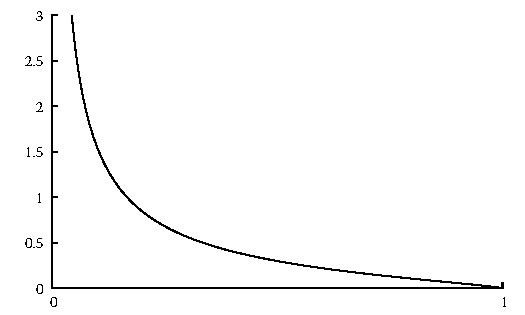
\includegraphics[width=\textwidth]{pdfPearsonXII}
\end{center}
\caption[Pearson XII distribution]{A J-shaped Pearson XII distribution, $\opr{Beta}(0, 1, \tfrac{1}{4}, 1\tfrac{3}{4})$}
\end{figure}

% ============================
\dist{Pearson II} (Symmetric beta) distribution~\cite{Pearson1895}: 
%
\begin{align}
\label{PearsonII}
\opr{PearsonII}(x\given \mu, b,\alpha) 
%&= \frac{1}{2s}\frac{\Gamma(2\alpha) }{ \Gamma(\alpha) } \Left(1-\frac{x^2}{4 s^2} \Right)^{\alpha-1} \\
&= \frac{1}{2^{2\alpha-1}  |b|}\frac{\Gamma(2\alpha) }{ \Gamma(\alpha)^2 } \Left(1-\Left(\frac{x-\mu}{ b}\Right)^2 \Right)^{\alpha-1}
\checked
 \\
& = \opr{Beta}(x\given \mu-b, 2b,\alpha, \alpha) 
\notag  \checked \\
& = \opr{GenBeta}(x\given \mu-b, 2 b ,\alpha, \alpha,1) \notag
\checked
\end{align}
A symmetric centered distribution with support $[\mu-b, \mu+b]$.

\begin{figure}[tp!]
\begin{center}
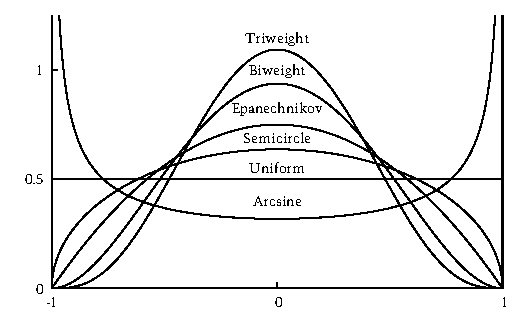
\includegraphics[width=\textwidth]{pdfPearsonII}
\end{center}
\caption[Pearson II distributions]{Special cases of the Pearson II distribution, $\alpha=\tfrac{1}{2}, 1, \tfrac{3}{2}, 2, 3, 4$.}
\end{figure}


% ============================
\dist{Arcsine} distribution~\cite{Norton1975}:
\begin{align}
\label{Arcsine}
\opr{Arcsine}(x\given a, s) &= \frac{1}{\pi |s| \sqrt{(\tfrac{x-a}{s}) (1-\frac{x-a}{s} )}} \checked \\
& =\opr{Beta}(x\given a,s,   \tfrac{1}{2},  \tfrac{1}{2}) \notag \checked \\
& =\opr{GenBeta}(x\given a,s, \tfrac{1}{2}, \tfrac{1}{2},1) \notag \checked
\end{align}
Describes the percentage of time spent ahead of the game in a fair coin tossing contest~\cite{Johnson1995,Norton1975}. The name comes from the inverse sine function in the cumulative distribution function,
$
\op{ArcsineCDF}(x\given 0,1) = \frac{2}{\pi} \op{arcsin}( \sqrt{x}) \checked
$.



 
% ============================
\dist{Central arcsine} distribution~\cite{Norton1975}: 
\begin{align}
\label{CentralArcsine}
\opr{CentralArcsine}(x\given b) &= \frac{1}{2 \pi  \sqrt{b^2-x^2}} \checked \\
%& =\opr{PearsonII}(x\given b, \tfrac{1}{2} ) \notag \\
& =\opr{Beta}(x\given b,-2b, \tfrac{1}{2}, \tfrac{1}{2})  \checked \notag \\
& =\opr{GenBeta}(x\given b,-2b, \tfrac{1}{2}, \tfrac{1}{2},1)  \checked \notag
\end{align}
A common variant of the arcsin, with support $x\in [-b,b]$ symmetric about the origin. Describes the position at a random time of a particle engaged in simple harmonic motion with amplitude $b$~\cite{Norton1975}. With $b=1$, the limiting distribution of the proportion of time spent on the positive side of the starting position by a simple one dimensional random walk~\cite{Feller1968}.\index{diffusion}


\dist{Semicircle} (Wigner semicircle, Sato-Tate) distribution~\cite{Wigner1955}
\begin{align}
\label{Semicircle}
\opr{Semicircle}(x\given b) &= \frac{2}{\pi b^2} \sqrt{b^2-x^2} \checked \\
& =\opr{Beta}(x\given -b, 2b, 1\tfrac{1}{2}, 1\tfrac{1}{2}) \notag \checked \\
& =\opr{GenBeta}(x\given -b, 2b, 1\tfrac{1}{2}, 1\tfrac{1}{2},1) \notag \checked
\end{align}
As the name suggests, the probability density describes a semicircle, or more properly a half-ellipse. This distribution arises as the distribution of eigenvectors of various large random symmetric matrices. 

\dist{Epanechnikov} (parabolic) distribution~\cite{Epanechnikov1969a}:
\begin{align}
\label{Epanechnikov}
\opr{Epanechnikov}(x\given \mu, b) 
&= \frac{3}{4} \frac{1}{|b|} \Left(1-\Left(\frac{x-\mu}{b}\Right)^2 \Right) \checked
 \\
& = \opr{PearsonII}(x\given \mu, b, 2) \notag \checked \\
& = \opr{Beta}(x\given \mu-b, 2 b, 2, 2) \notag   \checked \\
& = \opr{GenBeta}(x\given \mu-b, 2b, 2, 2,1) \checked \notag 
\end{align}
Used in non-parametric kernel density estimation.


\dist{Biweight} (Quartic) distribution:
\begin{align}
\label{Biweight}
\opr{Biweight}(x\given \mu, b) 
&= \frac{15}{16} \frac{1}{|b|} \Left(1-\Left(\frac{x-\mu}{b}\Right)^2 \Right)^2 
\checked
 \\
& = \opr{PearsonII}(x\given \mu, b, 3) \notag  \checked\\
& = \opr{Beta}(x\given \mu-b, 2 b, 3, 3) \notag   \checked \\
& = \opr{GenBeta}(x\given \mu-b, 2b, 3, 3,1)  \notag \checked
\end{align}
Used in non-parametric kernel density estimation.

\dist{Triweight} distribution:
\begin{align}
\label{Triweight}
\opr{Triweight}(x\given \mu, b) 
&= \frac{35}{32} \frac{1}{|b|} \Left(1-\Left(\frac{x-\mu}{b}\Right)^2 \Right)^3 
\checked
 \\
& = \opr{PearsonII}(x\given \mu, b, 4) \notag  \checked\\
& = \opr{Beta}(x\given \mu-b, 2 b, 4, 4) \notag   \checked \\
& = \opr{GenBeta}(x\given \mu-b, 2b, 4, 4,1)  \notag \checked
\end{align}
Used in non-parametric kernel density estimation.



\SSec{Interrelations}




The beta distribution describes the order statistics of a rectangular \eqref{Uniform} distribution.
\begin{align*}
\opr{OrderStatistic}_{\opr{Uniform}(a,s)} & (x \given \alpha, \gamma) =  \opr{Beta}(x\given a, s, \alpha, \gamma) \checked
\end{align*}
Conversely, the uniform \eqref{Uniform} distribution is a special case of the beta distribution. 
\begin{align*}
\opr{Beta}(x\given a, s, 1, 1) & = \opr{Uniform}(x\given a,s) \checked
\end{align*}



The beta and gamma distributions are related by
\[
\opr{StdBeta}(\alpha, \gamma) \sim \frac{\opr{StdGamma}_1(\alpha)} { \opr{StdGamma}_1(\alpha) + \opr{StdGamma}_2(\gamma) }
\checked
\notag
\]
which provides a convenient method of generating beta random variables, given a source of gamma random variables.


The Dirichlet distribution~\cite{Durbin1998,Gelman2004} is a multivariate generalization of the beta distribution. \index{Dirchlet distribution}

The beta distribution is a special case of the generalized beta distribution~\eqref{GenBeta}, and limits to the gamma distribution~\eqref{Gamma}.
\[
\opr{Gamma}(x\given a, \theta,\alpha)   \
& =  \lim_{\gamma\rightarrow\infty} \opr{Beta}(x\given a, \theta \gamma ,\alpha, \gamma ) \checked
\notag
\]
